\section{Principles of Nuclear Magnetic Resonance}

\begin{onehalfspace}
    \par Nuclear Magnetic Resonance (NMR) describes the behavior of atomic nuclei possessing non-zero spin in the presence of a strong static external magnetic field when they are perturbed by an additional oscillating magnetic field. This perturbation gives rise to an induced electromagnetic signal whose frequency depends on the local magnetic environment of the nuclei \citep{Rabi1938, blochNuclearInductionExperiment1946, haydenHistoryPhysicalPrinciples2016}. NMR is the fundamental physical principle underlying Magnetic Resonance Imaging \citep{currieUnderstandingMRIBasic2013, lauterburImageFormationInduced1973, mansfieldMultiplanarImageFormation1977} and will be discussed in further detail in this chapter.
\end{onehalfspace}

\subsection{Interaction of Nuclear Spins with a Static Magnetic Field}
\begin{onehalfspace}
    \par Protons and neutrons in an atomic nucleus possess intrinsic angular momentum associated with their quantum mechanical spin. This intrinsic angular momentum is commonly referred to as \textit{spin}. Hydrogen ($^{1}\!H$) is the nucleus most frequently investigated in NMR. It has a net nuclear spin quantum number $I=\tfrac{1}{2}$, which generates two discrete spin states characterized by the magnetic quantum numbers $M=\pm\tfrac{1}{2}$.
    \par Because nuclei carry electric charge, their spin gives rise to a magnetic dipole moment. In the absence of an external magnetic field, these magnetic moments are randomly oriented, resulting in no net macroscopic magnetization. When a static magnetic field $B_{0}$ is applied, the nuclear magnetic moments partially align with this field. Magnetic resonance arises from the interaction between the nuclear spin magnetic moments and $B_{0}$.
    \par Due to their angular momentum, the spin magnetic moments do not align perfectly parallel or antiparallel to the external field. Instead, they \textit{precess} around the direction of $B_{0}$ at a characteristic angular frequency known as the Larmor frequency $\omega_{0}$:
    \begin{equation}
        \omega_{0} = \gamma B_{0},
        \label{eq:larmor}
    \end{equation}
    where $\gamma$ is the gyromagnetic ratio, expressed in frequency per Tesla (for $^{1}\!H$, $\gamma = 42.57\ \text{MHz/T}$).
    \par For practical purposes, NMR typically considers the collective behavior of a large ensemble of spins rather than individual spins. A slight excess population of spins in the lower-energy state aligned with $B_{0}$ gives rise to a non-zero net magnetization vector $M_{0}$. This macroscopic magnetization is oriented along the direction of $B_{0}$ (conventionally the $z$-axis) and is proportional to both the population difference between the spin states and the magnitude of $B_{0}$.
\end{onehalfspace}

\subsection{NMR Signal}
\begin{onehalfspace}
    \par At thermal equilibrium, no time-varying signal is detected by the MR receiver coils because electromagnetic induction requires a component of the magnetization that lies in the plane transverse to $B_{0}$ and varies with time. Under equilibrium conditions, the net magnetization is purely longitudinal ($M_{z}$) and aligned with $B_{0}$, yielding no transverse component.
    \par To generate a detectable NMR signal in the presence of $B_{0}$, an additional magnetic field $B_{1}$ is applied to tip the equilibrium longitudinal magnetization $M_{z}$ away from the $z$-axis and thereby create a transverse magnetization component $M_{xy}$ (Figure \ref{fig:relaxation}). The field $B_{1}$ is created by a radiofrequency (RF) pulse that is applied orthogonally to $B_{0}$ and oscillating at the Larmor angular frequency $\omega_{0}$, thereby fulfilling the resonance condition and efficiently transferring magnetization into the transverse plane.

\par Under resonance conditions, the net magnetization vector is tipped by an angle $\alpha$ toward the transverse $x\text{-}y$ plane. The magnitude of this flip angle $\alpha$ is determined by both the duration ($\tau$) and the amplitude of the applied $B_{1}$ RF pulse:
\begin{equation}
    \alpha=\gamma B_{1}\tau\text{.}
\end{equation}

In the presence of such a pulse, the resulting magnetization can be decomposed into a longitudinal component, $M_{z}$, and a transverse component, $M_{xy}$, which arise from:
\begin{equation}
    M_{z}(0)=M_{0}\cos(\alpha)\text{,}
    \label{eq:mz}
\end{equation}
\begin{equation}
    M_{xy}(0)=M_{0}\sin(\alpha)\text{.}
    \label{eq:test}
\end{equation}

\par Consequently, full saturation of the net magnetization is achieved following the application of a \(90^\circ\) RF excitation pulse. Under these conditions, the equilibrium longitudinal magnetization \(M_{0}\) is completely rotated into the transverse plane, such that the transverse component \(M_{xy}\) attains a magnitude of \(M_{0}\), while the longitudinal component \(M_{z}\) is reduced to zero. In contrast, an inversion of the magnetization is produced by a \(180^\circ\) RF excitation pulse, also known as inversion pulse, which reverses the direction of the net magnetization vector, resulting in its alignment along the \(-z\) axis. 
\end{onehalfspace}

\begin{figure*}
   \centering
\begin{tabular}{m{3cm}m{3cm}m{3cm}}

\textbf{(a)}&\textbf{(b)}&\textbf{(c)}\\
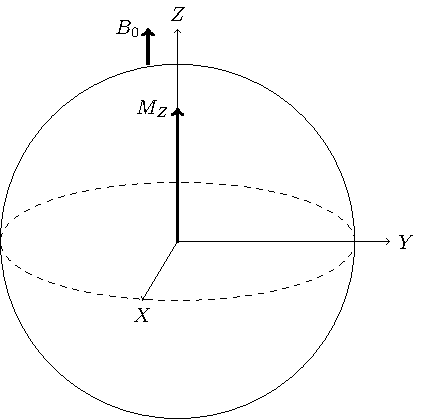
\includegraphics[width=3cm]{images/MRI-1.pdf}&
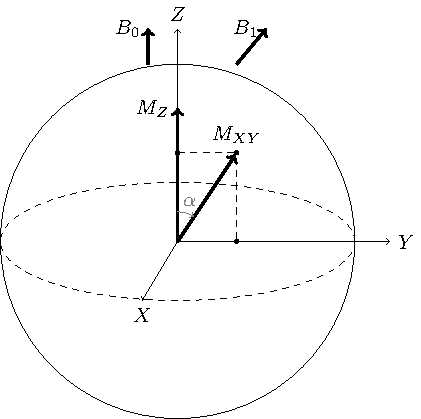
\includegraphics[width=3cm]{images/MRI-2.pdf}&
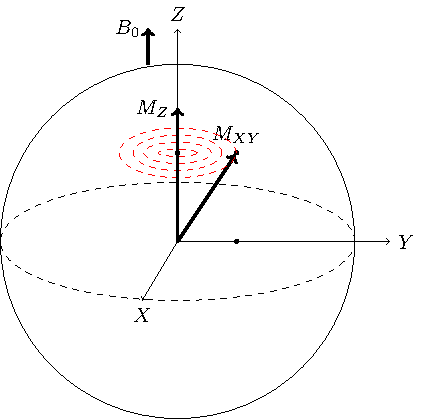
\includegraphics[width=3cm]{images/MRI-3.pdf}\\
\end{tabular}
    \caption[Generation of a Magnetic Resonance signal]{Generation of a magnetic resonance (MR) signal. \textbf{(a)} At thermal equilibrium, the longitudinal component of the net magnetization vector, $M_{z}$, is aligned parallel to the static magnetic field $B_{0}$. \textbf{(b)} Application of a radiofrequency (RF) pulse generates a time-varying magnetic field $B_{1}$, oriented orthogonally to $B_{0}$. This field induces a rotation of the magnetization vector from the longitudinal axis toward the transverse plane, giving rise to the transverse magnetization component $M_{xy}$. The flip angle of this rotation is determined by the amplitude and duration $\tau$ of the RF pulse. \textbf{(c)} Once the $B_{1}$ field is switched off, the transverse component $M_{xy}$ undergoes relaxation and decays, while the magnetization vector $M_{z}$ returns toward its equilibrium state aligned with $B_{0}$.}
    \label{fig:bmu}
\end{figure*}

\subsection{Spin relaxation}

\begin{onehalfspace}
    After a RF pulse is turned off, spins will precess toward the equilibrium magnetization by spin-lattice relaxation while also dephasing from one another due to spin-spin relaxation process (Figure \ref{fig:relaxation}). 
\end{onehalfspace}

\subsubsection{Spin-lattice relaxation ($T1$)}
\begin{onehalfspace}
    
Spin–lattice relaxation arises from the dissipation of absorbed energy by the spins as they return toward their equilibrium population distribution. Dipole–dipole interactions give rise to oscillatory magnetization dynamics that can be described by the Bloch equation \citep{blochNuclearInductionExperiment1946}:
\begin{equation}
\frac {d\text{\textbf{M}}}{dt}=\gamma(\text{\textbf{M}}\times\text{\textbf{B}})-\frac{(M_{z}-M_{0})\text{\textbf{k}}}{T_{1}}-\frac{M_{x}\text{\textbf{i}}+M_{y}\text{\textbf{j}}}{T_{2}}\text{.}
\label{eq:bloch}
\end{equation}

Solving this equation, the temporal evolution of the longitudinal magnetization \(M_z\) is given by:
\begin{equation}
    M_{z}(t)=M_{0}\left[1-(1-\cos(\alpha))e^{-t/T_{1}}\right]\text{,}
\end{equation}
where $t$ denotes the elapsed time following application of the RF pulse. The longitudinal magnetization $M_z$ recovers exponentially toward its equilibrium value $M_z(0)$ with a characteristic spin–lattice relaxation time constant $T_1$. The relaxation time $T_1$ varies as a function of tissue composition, temperature, and the magnetic field strength (e.g., gray matter 1.5T: $1,197 \pm 134$ ms, 3T: $1,607 \pm 11$ ms, 7T: $1,939 \pm 149$ ms; white matter 1.5T: $646 \pm 32$ ms, 3T: $838 \pm 50$ ms, 7T: $1,126 \pm 97$ ms  \citet{wrightWaterProtonT12008}).
\end{onehalfspace}

\subsubsection{Spin-spin relaxation ($T2$)}

\begin{onehalfspace}

Spin-spin relaxation arises from the loss of phase coherence between every spin as they return to equilibrium after the RF pulse. Spin-spin interactions induce magnetization dynamics in the transverse plane $M_{xy}$ that can be defined from the Bloch equation in \ref{eq:bloch} as follows:
\begin{equation}
    M_{xy}(t)=M_{0}\sin(\alpha)e^{-t/T_{2}}.
\end{equation}
In practice, $M_{xy}$ decays faster than $T_{2}$ with a true relaxation time constant $T_{2}^{*}$:
\begin{equation}
\frac{1}{T_{2}^{*}}=\frac{1}{T_{2}}+\frac{1}{T_{2}^{\prime}},
\end{equation}
where the parameters $T_{2}$, $T_{2}^{\prime}$ and $T_{2}^{*}$ also vary as a function of tissue composition, temperature, and magnetic field strength ( e.g., gray matter 1.5 T: $84.0 \pm 0.8$ ms, 3T: $1,607 \pm 11$ ms, 7T: $1,939 \pm 149$ ms; white matter 1.5T: $646 \pm 32$ ms, 3T: $838 \pm 50$ ms, 7T: $1,126 \pm 97$ ms \citet{petersT2MeasurementsHuman2007}).
\end{onehalfspace}

\begin{figure*}
   \centering
\begin{tabular}{m{6cm}m{6cm}}
(a)& (b)\\
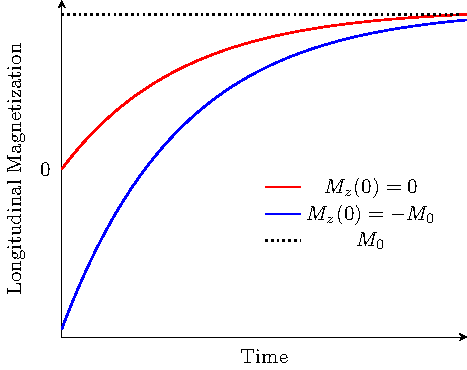
\includegraphics[width=6cm]{images/T1.pdf}&
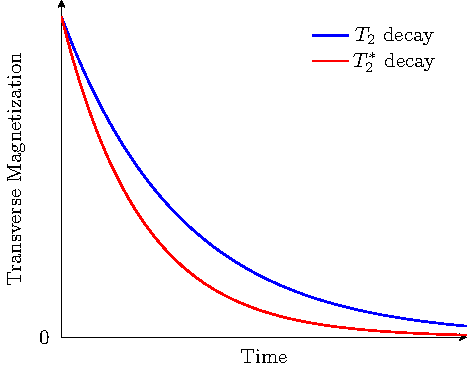
\includegraphics[width=6cm]{images/T2.pdf}\\
\end{tabular}
    \caption[Transverse and Longitudinal relaxations]{Transverse and Longitudinal relaxations. (a) Spin-Lattice relaxation of the longitudinal magnetization, $M_{z}$, with relaxation time constant $T_{1}$. Red line shows decay after an exitatory pulse ($\alpha = 90^{\circ}, M_{z}=0$), and blue line shows decay after and inversion pulse ($\alpha = 180^{\circ}, M_{z}=-M_0$). (b) Spin-spin relaxation of the transverse magnetization, $M_{xy}$. Red line shows $T_2^*$ decay, and blue line shows $T_2$ decay. $T_2^*$ decays faster because of $B_0$ inhomogeneities}
    \label{fig:relaxation}
\end{figure*}

\subsection{The Free Induction Decay Signal}

\begin{onehalfspace}
    \par When the RF pulse is turned off, the energy absorbed by spins is released as electromagnetic radiation following the lattice and longitudinal relaxations. The sum of relaxations create an oscillatory signal known as the Free Induction Decay (FID) signal, whose largest magnitude is when the RF pulse is turned off and then follows a rapidly decaying sine wave form with time constant $T_2^{*}$ (Fig. \ref{fig:FID}). 
    \par When imposing a magnetic field gradient during readout, the Larmor frequency varies linearly with position. To localize and encode the FID, the same frequency as the transmitted RF pulse is used to dephase it. Following low-pass filtering, the resulting complex signal has a bandwidth equal to the range of Larmor frequencies across the sample, enabling one‑dimensional spatial encoding..
\end{onehalfspace}

\begin{figure*}
   \centering
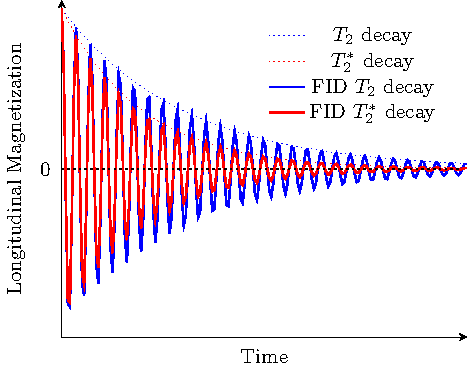
\includegraphics[width=6cm]{images/FID.pdf}
    \caption[Free Induction Decay Signal]{Free induction decay signal illustrating $T_{2}$, and $T_{2}^{*}$ relaxation decays in blue and red, respectively.}
    \label{fig:FID}
\end{figure*}

\subsection{Echoes}
\begin{onehalfspace}
    \par In most magnetic resonance (MR) experiments, the signal is acquired in the form of an echo, typically a spin echo or a gradient echo. Echo formation reverses the spin dephasing process and thereby increases the amplitude of the observable signal, which in turn makes echoes easier to measure than the free induction decay (FID) signal.

    \par Within a sample, individual nuclear spins precess at slightly different but constant Larmor frequencies. Spins with higher precessional frequencies accumulate a larger phase, $\phi$ as time evolves. After a time interval $t = \text{TE}/2$, application of a $180^{\circ}$ refocusing radiofrequency (RF) pulse inverts the spin phases to $-\phi$, causing them to continue precessing but in the opposite sense relative to their initial dephasing trajectory. Faster spins again accrue phase more rapidly, and this temporal evolution leads to a rephasing of the spin ensemble, i.e., a net phase coherence at time $t = \text{TE}$, associated with an increase in the transverse magnetization and thus in the measured signal. This rephased signal is termed an echo. When the echo is produced by a $180^{\circ}$ RF refocusing pulse, it is referred to as a spin echo, whereas when it is generated by appropriate manipulation of magnetic field gradients, it is known as a gradient echo.   
\end{onehalfspace}

\subsection{Gradient echo (GE)}
\begin{figure*}
   \centering
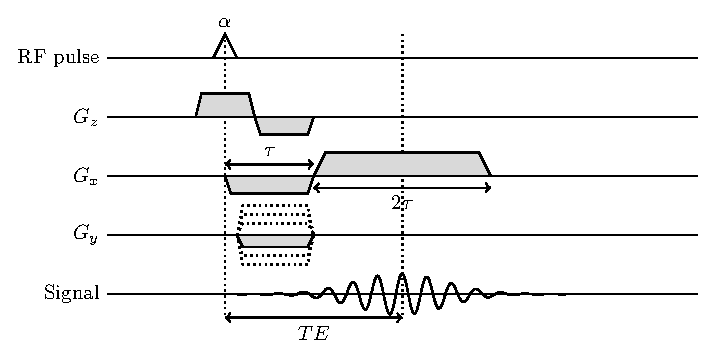
\includegraphics[width=10cm]{images/gradient_echo.pdf}
    \caption[Gradient echo pulse sequence]{Gradient-echo pulse sequence for a single phase-encoding step. This sequence is repeated with systematic variation in the polarity and amplitude of the phase-encoding gradients in order to sample multiple lines of $k$-space. Adapted from \citep{elsterGradientechoMRImaging1993}.}
    \label{fig:GE}
\end{figure*}
\begin{onehalfspace}
    \par Magnetic field gradients are produced by additional coils that superimpose a linear, direction‑dependent offset onto the static field $B_{0}$. Along a selected spatial direction, this offset causes the Larmor frequency to vary linearly with position ($\omega(\vec{r}) = \gamma (B_{0} + G \cdot r)$), thereby converting spatial location into a frequency label, this frequency variation is the basis for all spatial encoding in MRI. Gradient echoes (GE) are then generated by applying a gradient to dephase the transverse magnetization, followed by a second gradient of opposite polarity and appropriate amplitude to rephase it. Because this refocusing relies solely on gradients and does not correct for static $B_{0}$ inhomogeneities, the resulting signal decay reflects $T_{2}^{*}$ relaxation rather than $T_{2}$. Consequently, gradient-echo contrast is inherently $T_{2}^{*}$-weighted (Figure \ref{fig:GE}).

    \par In a typical GE sequence, an RF excitation pulse is applied in the presence of a slice-selection gradient $G_{z}$ to excite spins within a specific slice of the sample. Immediately following this, a gradient with opposite polarity to $G_{z}$ is applied to rephase the slice profile, ensuring that spins at the superior and inferior boundaries of the slice attain the same phase. Next, during an interval $\tau$, a frequency-encoding gradient along the $x$-direction is applied with negative polarity (corresponding to $-k_{x,\text{max}}$) to prephase the transverse magnetization, while a phase-encoding gradient along the $y$-direction shifts the signal to the desired $k_{y,n}$ value. Subsequently, a frequency-encoding gradient of opposite polarity and twice the area is applied over $2\tau$, during which the MR signal is sampled and fills the corresponding line in $k_{y}$-space. The gradient echo reaches its maximum amplitude at a time $\tau$ after the onset of the readout (frequency-encoding) gradient, which corresponds to the center of $k_{x}$ for that particular $k_{y}$ value \citep{elsterGradientechoMRImaging1993}.
\end{onehalfspace}

\section{Principles of Magnetic Resonance Imaging (MRI)}
\begin{onehalfspace}
    

Nuclear magnetic resonance (NMR) was initially employed to investigate chemical systems through their magnetic properties using magnetic resonance spectroscopy \citep{ernstApplicationFourierTransform1966}. Magnetic resonance imaging (MRI) emerged when it was proposed that two-dimensional MR images could be reconstructed from NMR principles by introducing spatial variations in the applied magnetic field across the sample \citep{mansfieldNMRDiffractionSolids1973, lauterburImageFormationInduced1973, haydenHistoryPhysicalPrinciples2016}.
\end{onehalfspace}
\subsection{Signal localization}
\label{sec:signal}

\subsubsection{Signal Localization with Magnetic Field Gradients}
\begin{onehalfspace}
To generate a MR image, the NMR signal must be acquired from different spatial locations. This spatial encoding is achieved by introducing controlled variations in the magnetic field, thereby creating spatially dependent Larmor frequencies. The application of small, well-defined magnetic field gradients superimposed on the main static field $B_0$ induces slight spatial variations in the precessional frequency. These linear gradients encode position along the $x$, $y$, and $z$ axes according to
\begin{equation}
    G_x = \frac{dB_x}{dx}, \quad
    G_y = \frac{dB_y}{dy}, \quad
    G_z = \frac{dB_z}{dz}.
\end{equation}

In the presence of such a magnetic field gradient, the total magnetic field at a given spatial location $\mathbf{r} = (x, y, z)$ can be expressed as
\begin{equation}
\begin{aligned}
    B(\mathbf{r})
    &= B_0 \ + \ xG_x \mathbf{i} \ + \ yG_y \mathbf{j} \ + \ zG_z \mathbf{k} \\
    &= B_0 \ + \ \mathbf{G_r} \cdot \mathbf{r},
\end{aligned}
\end{equation}
where $\mathbf{G_r} = (G_x,\, G_y,\, G_z)$ denotes the magnetic field gradient vector in units of mT/m generated by the gradient coils. The magnitude of the local magnetic field thus increases linearly with the distance of $\mathbf{r}$ from a chosen reference position.

According to Equation \ref{eq:larmor}, the Larmor (resonance) frequency of a spin is consequently position dependent:
\begin{equation}
\begin{aligned}
    \omega(\mathbf{r})
    &= \gamma B_0(\mathbf{r}) \\
    &= \gamma \bigl(B_0 + \mathbf{G_r} \cdot \mathbf{r}\bigr),
\end{aligned}
\label{eq:larmorreloaded}
\end{equation}
where $\gamma$ is the gyromagnetic ratio. Thus, when a radiofrequency (RF) pulse is applied in the presence of a magnetic field gradient, excitation is restricted to spins located within a specific spatial region that satisfies the corresponding resonance condition. Consequently, the resonance frequencies arising from the applied gradients are distributed across the bandwidth of the free induction decay (FID) signal, and this frequency dispersion is exploited to encode spatial information within the MR image.
\end{onehalfspace}

\subsubsection{Slice selection}
\begin{onehalfspace}
    
In MRI, nuclear spins are selectively excited within cross-sectional slices of a sample. Slices, typically oriented along the $z$-axis, are defined by applying a slice selective gradient field $G_z$ concurrently with the RF excitation pulse at the Larmor angular frequency $\omega_{0} = \gamma B_0$. The bandwidth of the RF pulse, $\Delta\omega$, determines the slice thickness $\Delta z$ according to
\begin{equation}
    \Delta z = \frac{\Delta \omega}{\gamma G_z}\text{,}
\end{equation}
where $\gamma$ denotes the gyromagnetic ratio. This pulse will only excite those spins within $z_{0} + \Delta z/2 \geq z \geq z_{0}-\Delta z/2$ , where the location of $z_{0}$ is defined by the carrier frequency of the pulse $\omega_{0}$ with respect
to the reference point of the magnet.

Thus, to obtain thinner slices, either the slice-select gradient amplitude must be increased, or the RF pulse bandwidth must be reduced. The latter requires a longer RF pulse duration and consequently may increase the overall scan time.
\end{onehalfspace}

\subsubsection{Frequency and phase encoding}

\begin{onehalfspace}
Spatial encoding within the slice is performed along the $x$- and $y$-axes by means of frequency encoding and phase encoding, respectively. During signal readout, frequency and phase encoding are used to map two-dimensional spatial information into the frequency domain for the slice-selectively excited spins. Frequency encoding of the spin density distribution is typically achieved with the gradient field $G_x$, while phase encoding is implemented using the gradient field $G_y$. 

Gradients acting on the transverse magnetization induce a position-dependent phase $\phi$ that accumulates over time as $\phi = \omega(x,y)t$, where
\begin{equation}
    \omega(x,y) = \gamma \left(B_0 + G_x x + G_y y\right)\text{,}
\end{equation}
By demodulating the signal at the Larmor angular frequency $\omega_0$, the baseband free induction decay (FID) signal at time $t$ arising from a voxel centered at $(x_0, y_0)$ with spatial extent $\Delta x \times \Delta y$ can be written as
\begin{equation}
    S(t) \propto \int_{x_0-\frac{\Delta x}{2}}^{x_0+\frac{\Delta x}{2}} \int_{y_0-\frac{\Delta y}{2}}^{y_0+\frac{\Delta y}{2}} \rho(x,y) \, e^{-i\gamma\left(G_x x + G_y y\right)t} \, \text{d}x \,\text{d}y\text{,}
    \label{eq:FDI}
\end{equation}
where $\rho(x,y)$ denotes the spin density distribution. 

Frequency encoding imparts a linear frequency variation along one spatial axis, $G_x$, while phase encoding applies a linear phase variation along the orthogonal axis, $G_y$. Together, they sample Cartesian k‑space line by line: frequency encoding fills each line along the readout direction during signal acquisition, and phase encoding steps increment the phase between acquisitions to traverse the orthogonal direction. The resulting two‑dimensional k‑space matrix is then transformed into image space via a single 2D inverse Fourier transform .
\end{onehalfspace}

\subsubsection{K-space}
\label{subsec:kspace}
\begin{onehalfspace}
    The spatial frequency domain resulting from frequency and phase encoding is referred to as the $k$-space \citep{mansfieldNMRDiffractionSolids1973, twiegKtrajectoryFormulationNMR1983}. Real-space coordinates $(x,y,z)$ are represented as spatial frequencies $(k_x,k_y,k_z)$ in the $k$-space. For the transverse directions, the $k$-space variables are defined as
    \begin{equation}
        k_x = -\gamma \int_0^t G_x(\tau)\,\text{d}\tau \approx -\gamma G_x t
    \end{equation}
    \begin{equation}
        k_y = -\gamma \int_0^t G_y(\tau)\,\text{d}\tau \approx -\gamma G_y t\text{,}
    \end{equation}
    assuming constant gradients over the readout interval. Under this formalism, the FID signal in \eqref{eq:FDI} can be rewritten as
\begin{equation}
    S(k_x,k_y) \propto \int \!\!\!\int \rho(x,y)\, e^{-i\left(k_x x + k_y y\right)} \,\text{d}x\,\text{d}y
    = \mathcal{F}\{\rho(x,y)\}\text{,}
    \label{eq:FDI2}
\end{equation}
where $\mathcal{F}\{\cdot\}$ denotes the two-dimensional Fourier transform. Hence, the spatial frequencies $(k_x,k_y)$ sampled by the signal $S$ correspond to the Fourier transform of the spin density distribution $\rho(x,y)$ at position $(x,y)$. 

A two-dimensional image of the spin density is then recovered by applying the inverse Fourier transform to the measured $k$-space data:
    \begin{equation}
    \rho(x,y) \propto \int \!\!\!\int S(k_x,k_y)\, e^{+i\left(k_x x + k_y y\right)} \,\text{d}k_x\,\text{d}k_y
    = \mathcal{F}^{-1}\{S(k_x,k_y)\}\text{.}
    \end{equation}

The $k$-space representation characterizes the spin density distribution under the influence of field inhomogeneities in a frequency–phase domain. In two-dimensional imaging, $k$-space sampling typically starts near the center of $k$-space, where low spatial frequencies (governing overall image contrast and gross structure) are encoded, and proceeds toward the periphery, where high spatial frequencies (governing image detail and edges) are acquired. Notably, each acquired line in $k$-space contributes information to the entire reconstructed MR image, rather than mapping to a single image line.
\end{onehalfspace}

\subsection{Echo Planar Imaging (EPI)}
\label{sec:epi}
\begin{figure*}
   \centering
\begin{tabular}{m{8cm}m{3cm}}
\textbf{(a)}&\textbf{(b)}\\
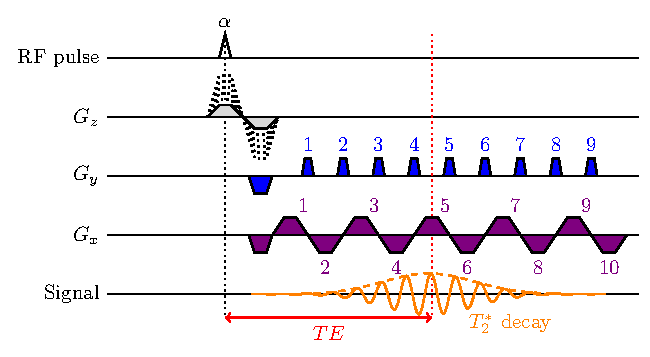
\includegraphics[width=8cm]{images/EPI.pdf}&
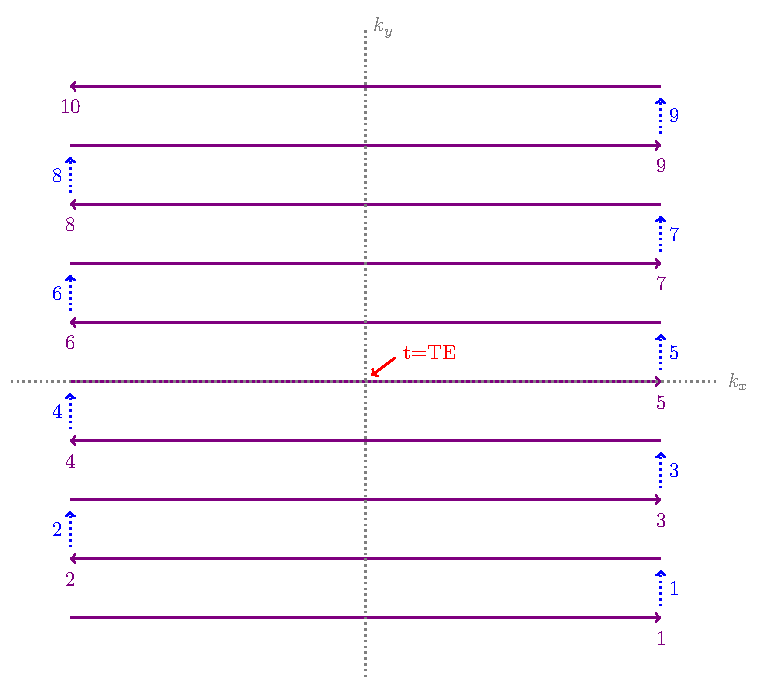
\includegraphics[width=3cm]{images/k-space.pdf}\\
\end{tabular}
    \caption[Echo Planar Imaging (EPI)]{\textbf{(a)} Echo-planar imaging (EPI) pulse sequence employing alternating readout gradients $G_x$ and phase-encoding gradients $G_y$ to achieve a rectilinear sampling trajectory in k-space. \textbf{(b)} Implementation using a Modulus-Blipped Echo-Planar Single-Pulse Technique to realize the corresponding k-space encoding.}
    \label{fig:epi}
\end{figure*}
\begin{onehalfspace}
Echo Planar Imaging (EPI) is a rapid MRI sequence designed to sample the entire $k$-space (or a substantial portion of it) during the course of a single $T_2^*$ decay, using either a single RF excitation pulse (single-shot EPI) or multiple excitations (multi-shot EPI) \citep{mansfieldMultiplanarImageFormation1977, stehlingEchoplanarImagingMagnetic1991}. Conventional gradient-echo acquisitions form a single echo at a time that is refer as the echo time (TE), and the FID has an amplitude that depends on $T_2^*$. As described in more detail in Chapter \ref{chap:fMRI}, multi-echo EPI sequences repeatedly sample the $T_2^*$ decay at multiple echo times.

In single-shot EPI, the $k$-space lines are traversed by rapidly alternating the readout gradient between positive and negative amplitudes following a single RF excitation (Fig. \ref{fig:epi}). Each lobe of the phase-encoding gradient $G_x$ above or below the baseline corresponds to a different $k_x$ line in $k$-space. In early implementations of the EPI sequence, a constant $G_y$ during readout produced a zig-zag trajectory through $k$-space, which led to reconstruction artifacts. The introduction of the Modulus Blipped Echo-Planar SIngle-pulse TEchnique echo-planar technique enabled sampling along a rectilinear trajectory in $k$-space by inserting small, discrete $G_y$ “blips” between successive readout gradient reversals, thereby incrementing $k_y$ in a controlled fashion \citep{ordidgeSnapshotImaging051989}. To increase spatial resolution and reduce distortion, multi-shot EPI partitions $k$-space acquisition across multiple RF excitation pulses, so that each shot covers only a subset (segment) of the full $k$-space \citep{barthSimultaneousMultisliceSMS2016,xuEvaluationSliceAccelerations2013,feinbergMultiplexedEchoPlanar2010}. 

EPI provides very high temporal efficiency but is constrained by the $T_2^*$ decay of the FID signal, gradient performance, and sensitivity to magnetic field inhomogeneities, which together limit the speed of $k$-space sampling. Still, owing its high temporal efficiency and sensitivity to $T_{2}^{*}$ changes, along with the continuous improvements in high performance gradient systems, EPI has become the main sequence for functional MRI studies.
\end{onehalfspace}